\documentclass[12pt]{article}
\usepackage{graphicx}
\usepackage{xcolor}
% \usepackage[margin=1.7cm]{geometry}
\usepackage{colortbl}
\usepackage{tikz}
\usepackage{amsmath}
\usepackage{caption}
\usepackage{subcaption}
\usepackage{textcomp}
\begin{document}
\begin{titlepage}
\begin{center}
    
\includegraphics[width=\textwidth]{./logo.png}
    \\ [2.5cm]
    \textsc{\Large Autonomous Mobile Robots}
    \\ [0.5cm]
    \textsc{\large Second assignment}
    \\ [1cm]
    \hrule
    \vspace{0.3cm}
    \textsc{Range Finder using Omnidirectional Camera}
    \\ [0.3cm]
    \hrule
    \vfill
    \textsc{Ruben Janssen, 10252657 \\ David van Erkelens, 10264019 \\ Laurens Verspeek, 10184465 \\[0.7cm] Department of Computer Science \\ University of Amsterdam \\[0.3cm] \today}
\end{center}
\end{titlepage}
\tableofcontents
\clearpage
\section{Introduction}
In this report, our findings regarding detecting distances from walls to our LEGO robot will be described. In mobile robotics, moving robots need to detect distances to walls in order to ensure a save navigation. Devices that are usually used to accomplish this task are laser range finders and ultrasonic detectors. These sensors operate by emitting a pulse and measuring the time the pulse needs to reflect on a surface and return to the emitter. For our LEGO robot, a omnidirectional camera is used.

\section{Setup}
The omnidirectional camera used consists of a standard webcam and a spherical mirror. The webcam is positioned to look upwards to the mirror, resulting in a 360\textdegree view of the surroundings of the robot. However, due to a lack of equipment, we have used a default image instead of a real-world camera. This has no impact however on the rest of the experiment, as the same principles apply.

\section{Processing the image}
In order to start working with the image, we have to flip the image. This is because the image is acquired with use of a camera, resulting in a upside-down image. As soon as the image is flipped, two calibration points have to be pointed out: the center of the image, in which the center of the camera lies, and the minimum distance, because the camera would otherwise detect itself. \\ \\
As soon as these points have been given, the image can be unwrapped into a new image in which every radial of the original image becomes a vertical line. If the calibration is correct, the border of the camera lens should be a straight line (as seen in figure c in section 4). The function used to unwrap this image takes a few arguments: the image to unwrap, the center of the image which is the center of the camera lens, the minimum and maximum distance and how many degrees should span one radial line. \\ \\
When the image is correctly unwrapped, the edges have to be detected. This can be done pretty easily. The unwrapped image will be converted into black and white, regarding a certain threshold. We have set this threshold at 200, converting every pixel which has a greyscale value lower than 200 to black and the others to white. Now, every border between black and white represents a wall in the original image. An example is shown in firgure d in section 4. \\ \\
Now the edges are detected, the distance to the edge has to be calculated. The distance in the image is only a pixel distance, this has to be converted into a real world distance. If we take $d$ as the real distance and $p$ as the distance in pixels. Then we'll take $\alpha$ as variable for the mirror shape and camera-mirror distance. The distance between the camera lens and the ground floor is defined as $h$. The relation between $p$ and $d$ then becomes:
\begin{equation}
	d(p) = h \tan{(\frac{p}{\alpha})}
\end{equation}
Please note that because we used the offline version, we had to estimate $\alpha$ amd $h$. We left $h$ at the default value, as it greatly change the result. Increasing or decreasing $h$ would only cause all calculated distances to differ, but the relative distances will still remain. We estimated $\alpha$ by doing some test runs, knowing that the detected edges were straight. As $\alpha$ stands for the curvature of the mirror, a wrong $\alpha$ would result into curved edges instead of straight edges. This way it was possible to estimate the value once the edges were detected correctly. \\ \\
However, the obtained image can be affected by noise and could thus contain an error in the distance measurement, which has to be quantified. Therefore, we have to calculate the uncertainty of the distances on the image plane to the metric distances on the ground floor. The error propagation law uses a first order Taylor expansion of the above relation:
\begin{equation}
\frac{\delta d(p)}{\delta p} = \frac{h}{\alpha} (1+\tan{(\frac{p}{\alpha})}^2)
\end{equation}
When a pixel distance error with a normal distribution of mean value $p$ and standard deviation $\sigma_p$ is assumed, the matric distance error has a normal distribution of mean value $d$ and standard deviation $\sigma_d$. According to the error propagation law, the standard deviation is then:
\begin{equation}
\sigma_d = \frac{\delta d(p)}{\delta p} \sigma_p
\end{equation}
From this, it can be seen that the further the point lies away from the robot, the more uncertain its location is. In the implementation however, we had to multiply this value with 0.1 as different units where using this calculatio (some values were propably in meters while others in centimeters).
\section{Testing}
We took one of our images and applied above matlab functions to it, the results are shown below.
\begin{figure}[h!]
	\centering
	\begin{subfigure}[b]{0.4\textwidth}
		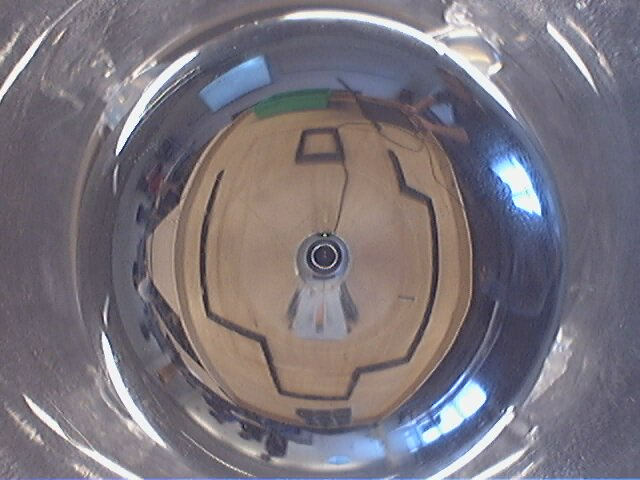
\includegraphics[width=\textwidth]{c.jpg}
		\caption{The image to process}
	\end{subfigure}
	~
	\begin{subfigure}[b]{0.4\textwidth}
		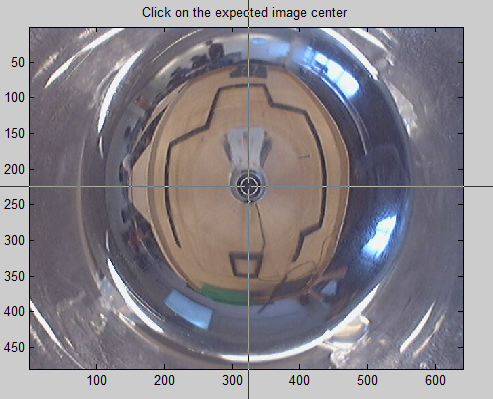
\includegraphics[width=\textwidth]{center.png}
		\caption{Determining the image center}
	\end{subfigure}

	\begin{subfigure}[b]{0.4\textwidth}
		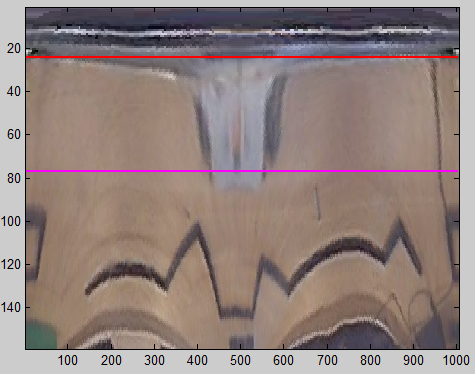
\includegraphics[width=\textwidth]{lines.png}
		\caption{Minimum and maximum distance}
	\end{subfigure}
	~
	\begin{subfigure}[b]{0.4\textwidth}
		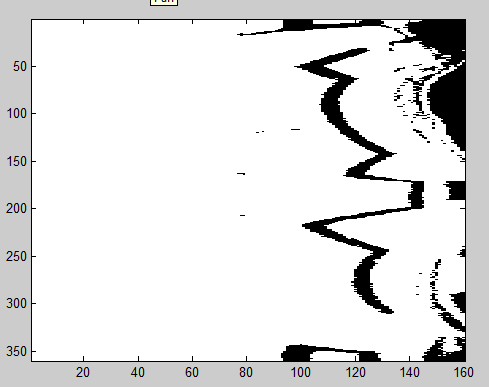
\includegraphics[width=\textwidth]{bw.png}
		\caption{The black and white mapping of the image}
	\end{subfigure}

	\begin{subfigure}[b]{0.4\textwidth}
		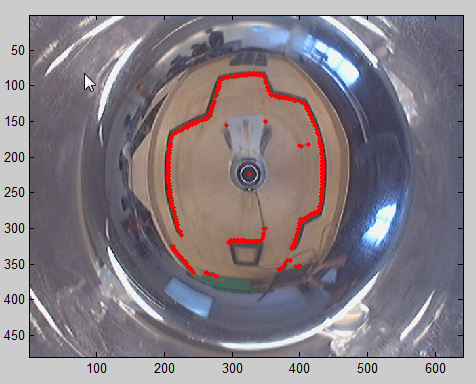
\includegraphics[width=\textwidth]{wallsinimg.png}
		\caption{The detected walls}
	\end{subfigure}
	~
	\begin{subfigure}[b]{0.4\textwidth}
		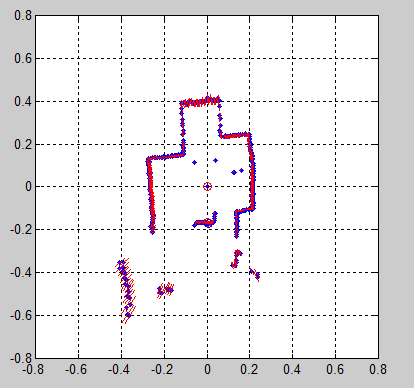
\includegraphics[width=\textwidth]{error.png}
		\caption{The error propagation}
	\end{subfigure}
\end{figure}
\clearpage
\section{Conclusion}
When looking at our test results, we can conclude that the method of detecting walls described above does a good job at detecting walls. Therefore, we can conclude that a robot can move savely through a building or maze with his algorithm implemented, keeping its bandwidth in mind.
\end {document}